\begin{egBox}{Verifying the Equivalence Relation for Components}[eg:25.1]
    Given \( X \), define an equivalence relation on \( X \) by setting 
    \( x \sim y \) if there is a connected subspace of \( X \) containing both
    \( x \) and \( y \).

    \baseSkip

    We can see that reflexivity (\( x \sim x \)) and symmetry (if 
    \( x \sim y \), then \( y \sim x \)) are both obvious; reflexivity follows
    by knowing that singleton sets are connected, and symmetry follows from
    our definition being symmetric.

    \baseSkip

    Now to verify the transitivity condition, let us start by assuming that 
    \( x \sim y \) and \( y \sim z \); this means that \( x \) and \( y \) are
    contained in a connected subspace \( A \) of \( X \), and \( y \) and 
    \( z \) are contained in a connected subspace \( B \) of \( X \).
    Since we know that \( A \) and \( B \) have a point in common (this point
    being \( y \)), it follows from [\hyperlink{thm:23.3}{Theorem 23.3}] that 
    \( A \cup B \) is a subspace of \( X \) that is also connected.
    Now because \( A \cup B \) contains \( x, y, \) and \( z \), we see that 
    \( x \sim z \), which verifies this condition.
\end{egBox}

\begin{egBox}{Verifying the Equivalence Relation for Path Components}[eg:25.2]
    Given \( X \), define an equivalence relation on \( X \) by setting 
    \( x \sim y \) if there is a path in \( X \) from \( x \) to \( y \).

    \baseSkip

    To show that this is an equivalence relation, we first not that if there 
    exists a path \( f: [ a, b ] \rightarrow X \) from \( x \) to \( y \)
    whose domain is the interval \( [ a, b ] \), then there is also a 
    path \( g \) from \( x \) to \( y \) having the closed interval 
    \( [ c, d ] \) as its domain; this follows from the fact that any two closed
    intervals in \( \mathbb{R} \) are homeomorphic.
    I.e., we are free to define a path using any closed interval as our 
    domain.

    \baseSkip
    
    Now, we have that reflexivity (\( x \sim x \)) holds for all \( x \in X \)
    due to the existence of a constant path \( f: [ a, b ] \rightarrow X \)
    defined by the equation \( f ( t ) = x \) for all \( t \).

    \baseSkip

    Symmetry (if \( x \sim y \), then \( y \sim x \)) follows from the fact that
    if \( f: [ 0, 1 ] \rightarrow X \) is a path from \( x \) to \( y \), then 
    the "reverse path" \( g: [ 0, 1 ] \rightarrow X \) defined by 
    \( g ( t ) = f ( 1 - t ) \) is a path from \( y \) to \( x \).

    \baseSkip

    Finally, transitivity is proved as follows: let 
    \( f: [ 0, 1 ] \rightarrow X \) be a path from \( x \) to \( y \), and 
    let \( g: [ 1, 2 ] \rightarrow X \) be a path from \( y \) to \( z \).
    We can "paste \( f \) and \( g \) together" to get a path 
    \( h: [ 0, 2 ] \rightarrow X \) from \( x \) to \( z \); the path \( h \)
    will be continuous by the "pasting lemma", that is by
    [\hyperlink{thm:18.3}{Theorem 18.3}].
\end{egBox}

\begin{egBox}{T vs. t}[eg:25.3]
    Show that a lower-case t is not homeomorphic to an upper-case T.
    Think of each as the union of two closed line segments (no thickness)
    in \( \mathbb{R}^{ 2 } \) with the subspace topology.

    \baseSkip 

    Towards a contradiction, assume that there exists a homeomorphism
    \( f: t \rightarrow T \).

    \begin{figure}[H]
        \centering
        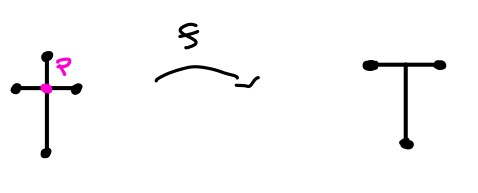
\includegraphics[ width = 0.5\linewidth ]{figures/Section 25/eg25-3.jpg}
        \caption{The two subspaces}
        \label{fig:25-3-1}
    \end{figure}
    There is a restricted homeomorphism that we can consider:
    \( g: t \setminus \{ p \} \rightarrow T \setminus \{ f ( p ) \} \).
    Notice that \( g \) is still a homeomorphism since domain/codomain 
    restrictions of continuous functions are still continuous.

    \baseSkip 

    We see that t has four connected components with \( \{ p \} \) removed.
    However, for T, we see that we can have at most three connected components.
    Thus, we know that t and T cannot be homeomorphic since they should have
    the same number of connected components otherwise.
\end{egBox}

\begin{egBox}{Connected Components are Not Always Open}[eg:25.4]
    Consider the topologist's sine curve \( \mathcal{S} \), or really, 
    consider the subspace \( \hat{ \mathcal{S} } \) obtained by cropping 
    \( \mathcal{S} \) as shown in Figure (\ref{fig:25-4-1}).

    \begin{figure}[H]
        \centering
        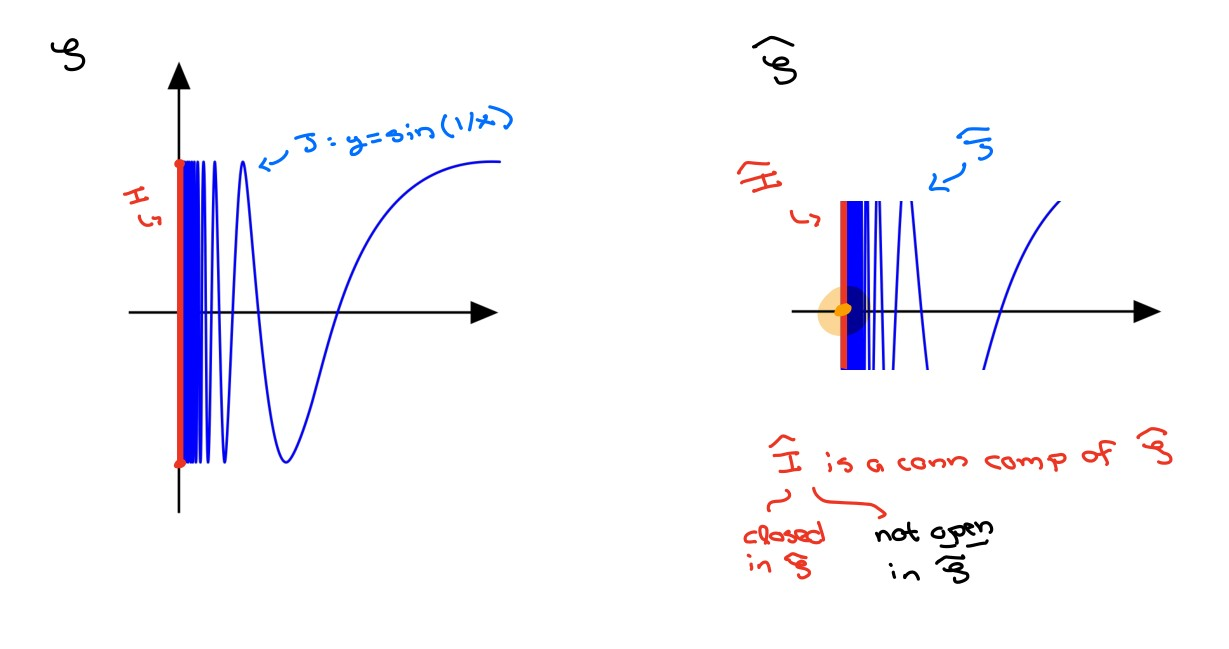
\includegraphics[ width = 0.6\linewidth ]{figures/Section 25/eg25-4.jpg}
        \caption{The two subspaces in question}
        \label{fig:25-4-1}
    \end{figure}

    We can see that this cropping results in \( \hat{ \mathcal{S} } \) to be 
    composed up of connected components; in particular, we see that 
    \( \hat{ I } \) is a connected component of \( \hat{ \mathcal{S} } \).
    We know that \( \hat{ I } \) is closed in \( \hat{ \mathcal{S} } \), but,
    \( \hat{ I } \) is not open in \( \hat{ \mathcal{S} } \) since any 
    neighborhood of any point in \( \hat{ I } \) is not entirely contained in
    \( \hat{ I } \).
\end{egBox}

\begin{egBox}{Locally Connected}[eg:25.5]
    Topologist's sine curve is not locally connected; using the same
    argument as in the [\hyperlink{eg:25.4}{previous example}].
    However, we see that \( \mathbb{R} \) is locally connected.

    \begin{figure}[H]
        \centering
        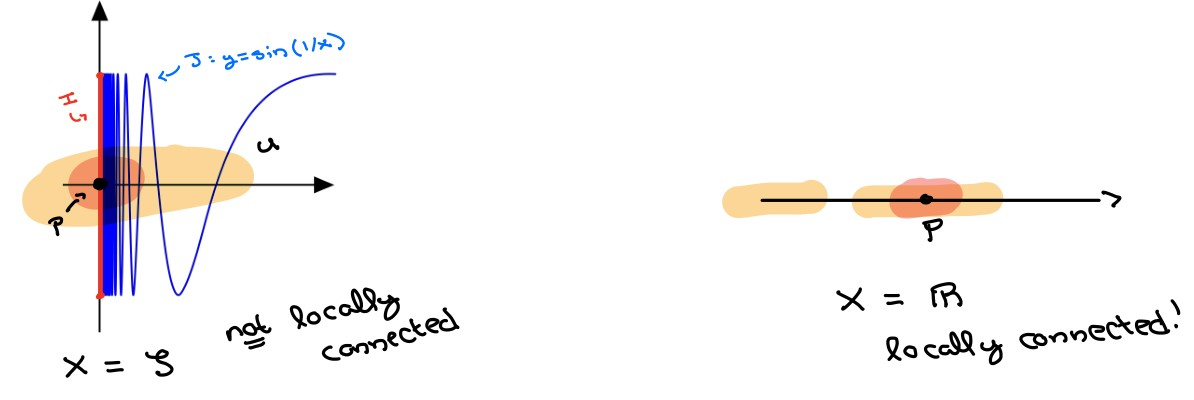
\includegraphics[ width = 0.8\linewidth ]{figures/Section 25/eg25-5.jpg}
        \caption{The two subspaces in question}
        \label{fig:25-5-1}
    \end{figure}
\end{egBox}

\begin{egBox}{Connected Components of \( \mathbb{R}_{ \ell } \)}[eg:25.6]
    Let \( \mathbb{R}_{ \ell } \) be \( \mathbb{R} \) with the lower-limit
    topology.
    Find its connected components.

    \baseSkip

    Let \( p \in \mathbb{R}_{ \ell } \) be given.
    Let \( C ( p ) \) be the connected component containing \( p \).
    Recall that the connected component is the union of all connected subspaces
    of \( \mathbb{R}_{ \ell } \) containing \( p \) itself.
    We claim that \( C ( p ) = \{ p \} \).

    \baseSkip

    For any \( a < p \), we see that \( [ a, p ) \cap C ( p ) \) is itself
    clopen in \( C ( p ) \) under the subspace topology since we know that
    \( [ a, p ) \) is clopen in \( \mathbb{R}_{ \ell } \).
    However, \( [ a, p ) \cap C ( p ) \) cannot equal to \( C ( p ) \) since
    \( [ a, p ) \) does not contain \( p \).
    Because \( C ( p ) \) is connected, we see that the intersection must be 
    \( \emptyset \), so we see that \( a \notin C ( p ) \).
    I.e., if we have that \( a < p \), then \( a \) is not in \( C ( p ) \).

    \baseSkip

    Now if \( a > p \), then we can consider the interval \( [ a, a + 1 ) \).
    We see that \( [ a, a +1 ) \cap C ( p ) \) is clopen in \( C ( p ) \)
    under the subspace topology, but again not equal to \( C ( p ) \) since
    \( [ a, a + 1 ) \) does not contain \( p \).
    Thus, we have that the intersection must be \( \emptyset \).
    As a results we also find that \( a \notin C ( p ) \). 
    I.e., if we have that \( a > p \), then \( a \) is not in \( C ( p ) \).
    
    \baseSkip 

    From this, we see that \( C ( p ) \) must be \( \{ p \} \), which tells us
    that \( \mathbb{R}_{ \ell } \) is very disconnected.
\end{egBox}